% Indicate the main file. Must go at the beginning of the file.
% !TEX root = ../main.tex

%%%%%%%%%%%%%%%%%%%%%%%%%%%%%%%%%%%%%%%%%%%%%%%%%%%%%%%%%%%%%%%%%%%%%%%%%%%%%%%%
% 02_methods
%%%%%%%%%%%%%%%%%%%%%%%%%%%%%%%%%%%%%%%%%%%%%%%%%%%%%%%%%%%%%%%%%%%%%%%%%%%%%%%%

\section{Methods}
\label{methods}

\subsection{Data}%%%%%%%%%%%%%%%%%%%%%%%%%%%%%%%%%%%%%%%%%%%%%%%%%%%%%%%%%%%%%%%

The used data for this project is the SwissImage RS \autocite{swisstopoSWISSIMAGERS2024}
data from the Swiss Federal Office of Topography (SwissTopo).
It is a raster dataset with a resolution of 0.1m containing four bands: RGB and NIR.
In order to cover the area of interest (AOI) 6 tiles of the dataset are needed.
Over this large AOI there are three areas labeled with the corresponding labels \autoref{fig:aoi_labeled}.
These labels were provided by a team of researchers from the ZHAW. The three
areas are distributed over a residential area (83487m\textsuperscript{2}),
an industrial area (132642m\textsuperscript{2}) and a rural area (82740m\textsuperscript{2}).
Two kinds of labels are available: The land cover category \autoref{fig:category_areas} and an assessment of the 
degree of perviousness \autoref{fig:sealed_areas}. In \autoref{fig:label_distribution} the distribution of
the data available for each label is shown for both the land cover category (\texttt{category}) and the sealing assessment (\texttt{sealed}).
A third kind of labels was generated by simplifying the degree of perviousness into two classes: pervious and impervious (\texttt{sealed\_simple}).
This was done by reclassifying the unknown areas to sealed ones since they only consist of BuildingDistortions and
ConstructionSites.

\begin{figure}[H]
    \centering
    \captionsetup{width=0.8\linewidth}
    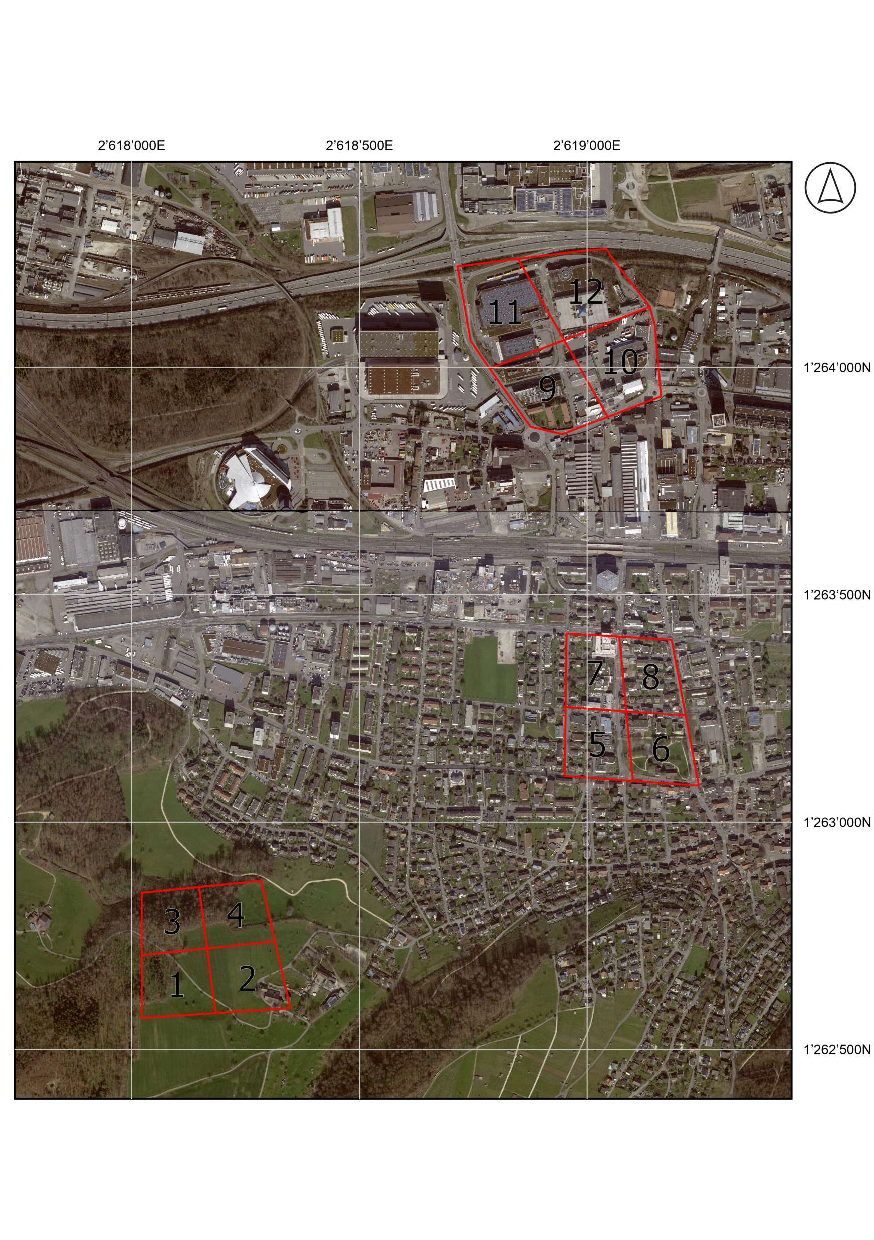
\includegraphics[scale=0.9, trim=-1.1cm 2cm 0cm 2cm, clip]{figures/map_aoi.pdf}
    \caption{Map of the AOI, Pratteln, a  municipality in the canton of Basel-Landschaft, Switzerland. 
    The three marked areas, each split in four tiles, are the areas with corresponding labels. 1 - 4 are in the rural area,
    5 - 8 in the residential area and 9 - 12 in the industrial area.}
    \label{fig:aoi_labeled}
\end{figure}

\begin{figure}[H]
    \centering
    \captionsetup{width=0.8\linewidth}
    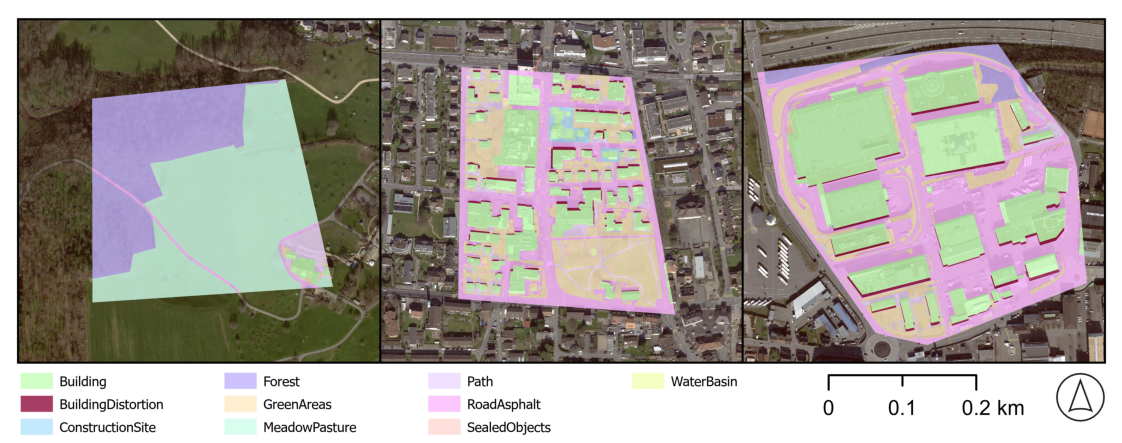
\includegraphics[width=\linewidth]{figures/map_aoi_category.pdf}
    \caption{The three areas with the corresponding land cover categories.}
    \label{fig:category_areas}
\end{figure}

\begin{figure}[H]
    \centering
    \captionsetup{width=0.8\linewidth}
    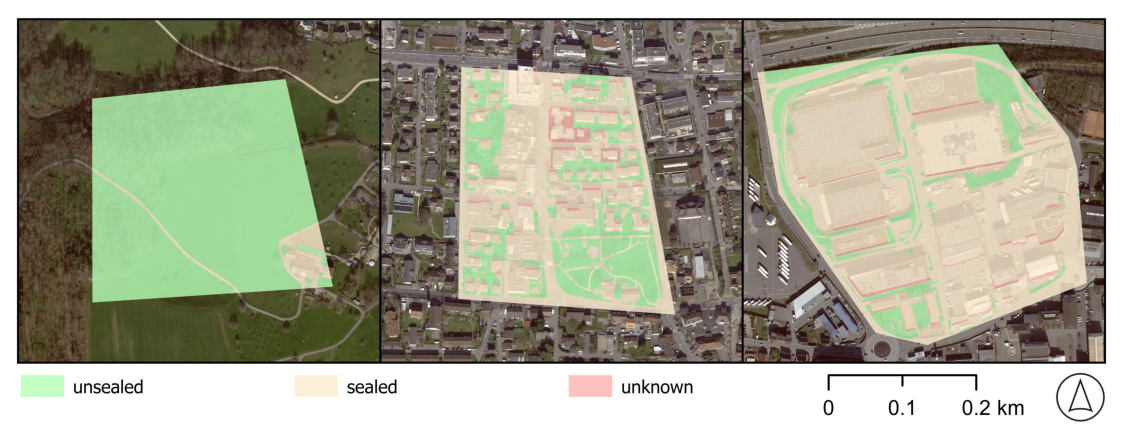
\includegraphics[width=\linewidth]{figures/map_aoi_sealing.pdf}
    \caption{The three areas with the corresponding degree of perviousness.}
    \label{fig:sealed_areas}
\end{figure}

\begin{figure}[H]
    \centering
    \captionsetup{width=0.8\linewidth}
    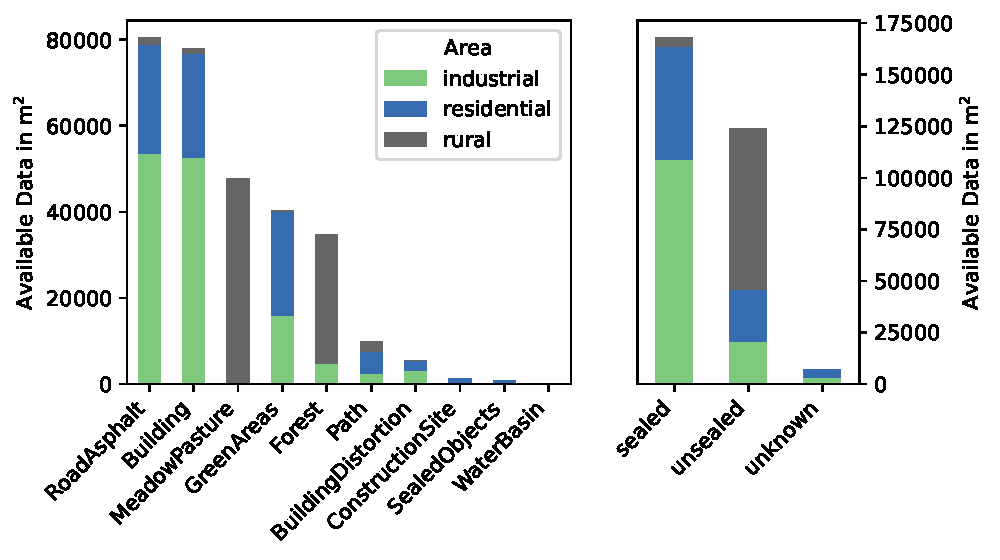
\includegraphics{figures/area_by_category_and_seal.pdf}
    \caption{Available data by label, colored by the area.}
    \label{fig:label_distribution}
\end{figure}


\subsection{Programming Language and Frameworks}%%%%%%%%%%%%%%%%%%%%%%%%%%%%%%%%

To build and train the deep learning model, the programming language Python was used.
The Frameworks PyTorch and Lightning are widely used and powerful tools for building
deep learning models.


\subsection{Model Architecture}%%%%%%%%%%%%%%%%%%%%%%%%%%%%%%%%%%%%%%%%%%%%%%%%%

For this study, an adapted version of the ResNet-18 architecture was employed to classify 
aerial imagery with high spatial resolution. ResNet-18 is a Convolutional Neural Network 
(CNN) model widely recognized for its residual connections, which mitigate the vanishing 
gradient problem during training. These connections allow for deeper networks while 
maintaining efficient backpropagation.

To suit the unique requirements of this research, several modifications were made to the 
standard ResNet-18 architecture:

\begin{itemize}
    \item \textbf{Input Channels}: The original ResNet-18 was modified to accept four input 
    channels (e.g., red, green, blue, and near-infrared bands) instead of the default 
    three channels (RGB). This adjustment allows the model to leverage the additional 
    spectral information for improved classification performance on remote sensing data.

    \item \textbf{Layer Configuration}: The network consists of three stages, with 
    residual blocks containing two convolutional layers per block. The layer configuration 
    was defined as \texttt{[2, 2, 2]}, corresponding to the number of residual blocks in 
    each stage.

    \item \textbf{Output Design}: The model was tailored for pixel-wise classification 
    tasks. The final fully connected layer was replaced with a convolutional layer to 
    output class probabilities over a patch of pixels. The size of the output patch is 
    adjustable via the \texttt{output\_patch\_size} parameter.

    \item \textbf{Pooling and Feature Extraction}: An adaptive average pooling layer was 
    utilized to condense spatial features while maintaining flexibility in input 
    dimensions. This pooling layer ensures compatibility with variable input sizes.

    \item \textbf{Regularization and Initialization}: Batch normalization layers were used 
    to stabilize training and improve generalization. Weights in the convolutional layers 
    were initialized using Kaiming normal initialization, enhancing the model's 
    convergence during training.

    \item \textbf{Optimization and Training}: The model was trained using the AdamW 
    optimizer, which combines adaptive learning rate methods with weight decay for 
    regularization. A weighted cross-entropy loss function was employed to handle class 
    imbalances effectively.
\end{itemize}

The modified ResNet-18 model was implemented using PyTorch and integrated into the 
Lightning framework for efficient training and evaluation. The design leverages the 
contextual and spectral richness of the four-channel input data, making it well-suited 
for pixel-level surface sealing classification tasks.

\subsection{Data Processing and Augmentation}%%%%%%%%%%%%%%%%%%%%%%%%%%%%%%%%%%

To feed data into the neural network, it is necessary to process it into a format that can be used for training.
A standardized sample size is needed to ensure that the model can be trained on the data.


\subsubsection{Preprocessing}%---------------------------------------
In a first step the data was processed using ArcGIS Pro. The process included a few steps implemented as
a model with the Model Builder \autoref{fig:processing_model}. The 6 tiles where mosaicked together and the area of interest 
was clipped. The area labels 1 - 12 and both versions of available data labels where transformed to raster datasets
and added as additional bands to the dataset. The data was then exported as a GeoTIFF file.
In order to use the data in a neural network an additional step was necessary. Using Python,
the data was transformed into Zarr format. This format is a chunked, compressed, N-dimensional array
storage format with multi-scale support. This allows for lazy loading and therefore for a more memory
efficient data access during training.

\begin{figure}[H]
    \centering
    \captionsetup{width=0.8\linewidth}
    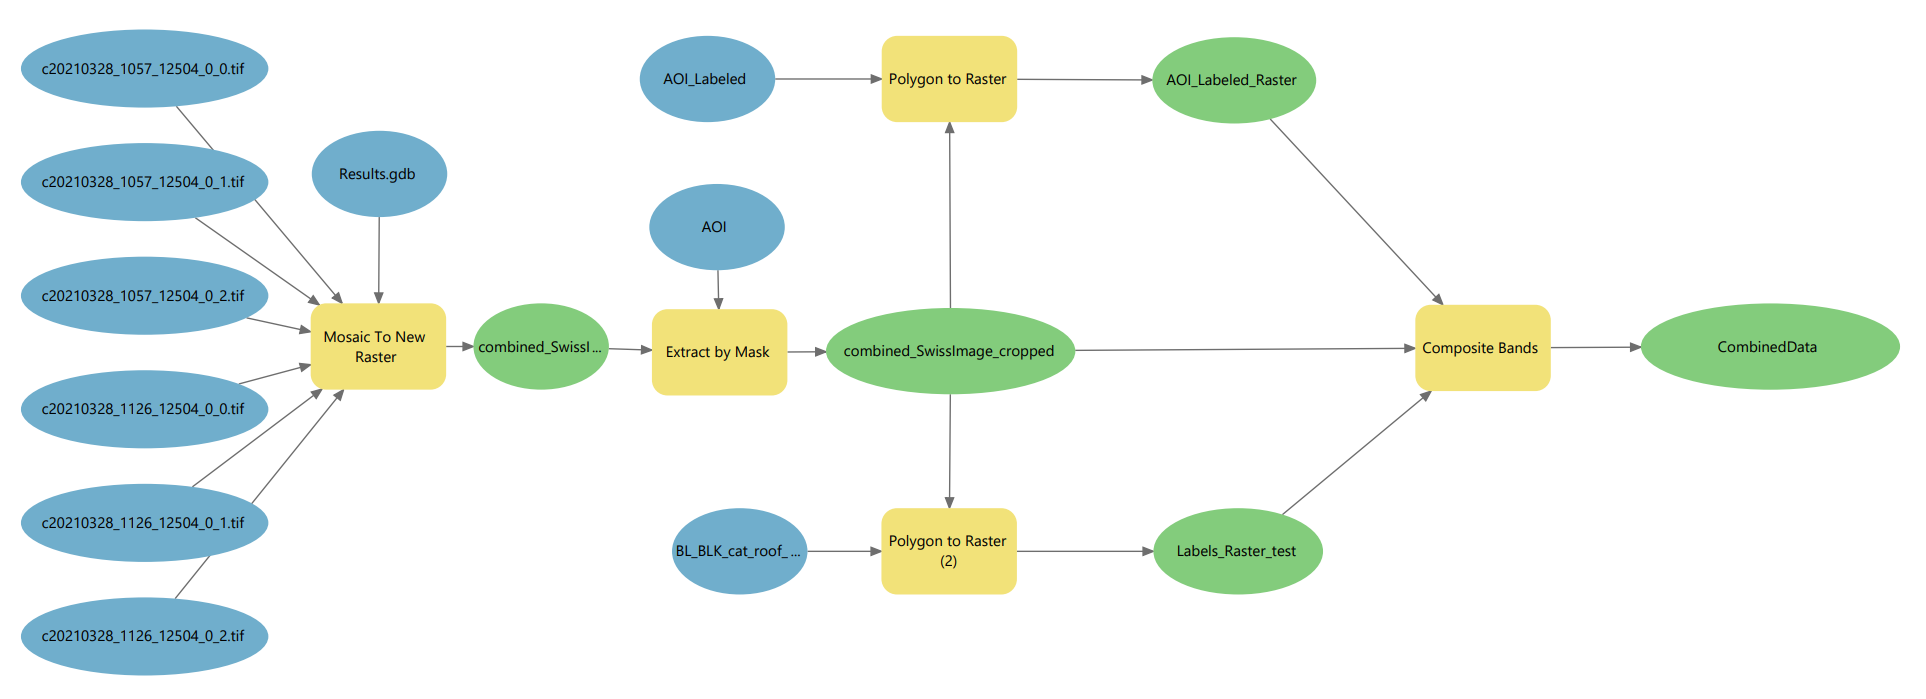
\includegraphics[width=\linewidth]{figures/ArcGIS_Model.png}
    \caption{ArcGIS model used for preprocessing the data.}
    \label{fig:processing_model}
\end{figure}


\subsubsection{Processing and Augmentation}%-------------------------------

To feed the data into a neural network a PyTorch DataLoader was implemented.
The data was sampled as cutouts of size 51x51 pixels, predicting the 5x5 center pixels as output.
This cutout size and output size where implemented as a parameter 
but no other values where tested.
The DataLoader indexes the available data depending on the cutout size and the 
corresponding area labels depending on the purpose:

\begin{tabular}{ll}
    \hspace{1.2em}\textbullet\ Areas for Training:   & 1, 2, 5, 6, 9, 10 \\
    \hspace{1.2em}\textbullet\ Areas for Validation: & 3, 7, 11          \\
    \hspace{1.2em}\textbullet\ Areas for Testing:    & 4, 8, 12          \\
\end{tabular}

It handles the data augmentation on the fly, during training steps.
For the data augmentation a parent class BaseAugmentor was implemented from which the different augmenters inherit. 
The implemented augmentors - refer to \autoref{tab:augmentors} - are then chained into a object of the class AugmentorChain
which can be used in the DataLoader. Only the Flip- and RotateAugmentor where used for the training of the models.


\begin{table}[H]
    \centering
    \caption{Implemented augmentors}
    \label{tab:augmentors}
        \begin{tabular}{ll}
        \toprule
        \textbf{Augmentor} & \textbf{Description} \\
        \midrule
        FlipAugmentor & Randomly flips the image vertically and horizontally\\
        RotateAugmentor & Randomly rotates the image 0, 90, 180 or 270° \\
        PixelNoiseAugmentor & Adds random noise to the image (parameter: scale) \\
        ChannelNoiseAugmentor & Adds random noise to the channels (parameter: scale) \\
        \bottomrule
        \end{tabular}
\end{table}


\subsection{Fitting the Model}%%%%%%%%%%%%%%%%%%%%%%%%%%%%%%%%%%%%%%%%%%%%%%%%%

Fitting the model was done on the IUNR HPC cluster using node 301 a HPE Apollo 6500 Gen10+ 
node running Rocky Linux 8. The node is equipped with 8 NVIDIA L40S GPUs (48GB each), 
dual AMD EPYC 7742 processors, 512 cores, and 5800 GB of storage, 
providing the computational power needed for high-performance tasks.
The training was done using a potential limit of 300 epochs and an early stopping Callback
set to stop after 10 epochs without improvement. Batch size was set to 128 for training and 256 for validation and prediction.
During training only the best model and the last model where saved.
On completion of the training the best model was loaded and used for prediction on the whole dataset.
This predictions where saved as a Zarr file for later use in the evaluation.
For each the category classification and the perviousness classification two models where trained
with and without data augmentation. The data augmentation was done using the Flip- and RotateAugmentor.
The learning rate was set to 0.001 and weight decay to 0.01.

For the simplified perviousness classification a limited hyperparameter search was done.
All combinations of the following parameters where tested:

\begin{tabular}{ll}
    \hspace{1.2em}\textbullet\ Learning rate:       & 0.001, 0.0001                                \\
    \hspace{1.2em}\textbullet\ Weight decay:        & 0, 0.1, 0.01                                 \\
    \hspace{1.2em}\textbullet\ Data augmentation:   & no augmentation, Flip- and RotateAugmentor    \\
\end{tabular}


\subsection{Evaluation}%%%%%%%%%%%%%%%%%%%%%%%%%%%%%%%%%%%%%%%%%%%%%%%%%%%%%%%%

For the performance evaluation of the models, the Python library Scikit-Learn was used. 
The predictions where loaded from the Zarr file and compared to the ground truth labels.
Accuracy, F1-Score weighted and per class where calculated for every model and stored to a CSV file
for later comparison. For the best model the accuracy was as well calculated grouped per
corresponding land cover category to provide insight which category was classified best.